% Template created by Karol Kozioł (www.karol-koziol.net) for ShareLaTeX

\documentclass[a4paper,9pt]{extarticle}
\usepackage[utf8]{inputenc}
\usepackage[T1]{fontenc}
\usepackage{graphicx}
\usepackage{xcolor}
\usepackage{tikz,float}
\usepackage{booktabs}
\usepackage{amsmath,amssymb,textcomp}
\everymath{\displaystyle}

\usepackage{times}
\renewcommand\familydefault{\sfdefault}
\usepackage{tgheros}
\usepackage[defaultmono,scale=0.85]{droidmono}

\usepackage{multicol}
\setlength{\columnseprule}{0pt}
\setlength{\columnsep}{20.0pt}


\usepackage{geometry}
\geometry{
a4paper,
total={210mm,297mm},
left=10mm,right=10mm,top=10mm,bottom=15mm}

\linespread{1.3}


% custom title
\makeatletter
\renewcommand*{\maketitle}{%
\noindent
\begin{minipage}{0.4\textwidth}

\begin{tikzpicture}
\node[rectangle,rounded corners=6pt,inner sep=10pt,fill=blue!50!black,text width= 0.95\textwidth] {\color{white}\Huge \@title};
\end{tikzpicture}
\end{minipage}
\hfill
\begin{minipage}{0.55\textwidth}
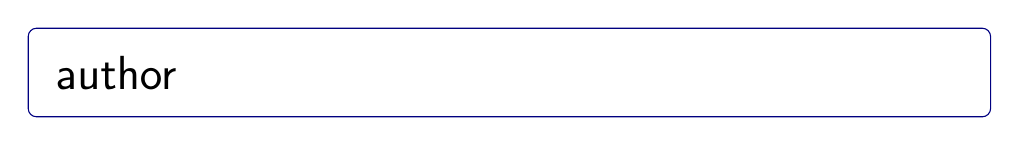
\begin{tikzpicture}
\node[rectangle,rounded corners=3pt,inner sep=10pt,draw=blue!50!black,text width= 0.95\textwidth] {\LARGE \@author};
\end{tikzpicture}
\end{minipage}
\bigskip\bigskip
}%
\makeatother

% custom section
\usepackage[explicit]{titlesec}
\newcommand*\sectionlabel{}
\titleformat{\section}
  {\gdef\sectionlabel{}
   \normalfont\sffamily\Large\bfseries\scshape}
  {\gdef\sectionlabel{\thesection\ }}{0pt}
  {
\noindent
\begin{tikzpicture}
\node[rectangle,rounded corners=3pt,inner sep=4pt,fill=blue!50!black,text width= 0.95\columnwidth] {\color{white}\sectionlabel#1};
\end{tikzpicture}
  }
\titlespacing*{\section}{0pt}{15pt}{10pt}


% custom footer
\usepackage{fancyhdr}
\makeatletter
\pagestyle{fancy}
\fancyhead{}
\fancyfoot[C]{\footnotesize \textcopyright\ \@date\ \ \@author}
\renewcommand{\headrulewidth}{0pt}
\renewcommand{\footrulewidth}{0pt}
\makeatother


\title{Aeronautics Formula Sheet}
\author{compiled by Lucas Alava Pe\~{n}a}%
\date{2017}



\begin{document}
\renewcommand{\arraystretch}{1.5}

\maketitle

\begin{multicols*}{2}



\section{Aircraft Geometry}
\begin{tabular}{ll}
Wing taper ratio & $\lambda=\frac{c_t}{c_r}$\\
Standard mean chord (SMC) & $\bar{c}=\frac{S}{b}$\\
Aspect ratio (AR) & $AR=\frac{b}{\bar{c}}=\frac{b^2}{S}$\\
Mean aerodynamic chord (MAC) & $\bar{\bar c}=\frac{1}{S} \int_{-\frac{b}{2}}^{\frac{b}{2}} c^2 (y) dy$
\end{tabular}





\section{Lift \& Airfoils}
\begin{tabular}{ll}
Lift & $L=\frac{1}{2}{\rho}_{\infty} {V_{\infty}}^2 S C_L$\\
Reynolds number (Re) & $Re = \frac{\rho V_{\infty} c}{\mu}$\\
Coefficient of Lift & $C_L=\frac{L}{\frac{1}{2}{\rho}_{\infty} {V_{\infty}}^2 S}$\\
Coefficient of Drag & $C_D=\frac{D}{\frac{1}{2}{\rho}_{\infty} {V_{\infty}}^2 S}$\\
Pitching Moment Coefficient & $C_M=\frac{M}{\frac{1}{2}{\rho}_{\infty} {V_{\infty}}^2 S c}$\\
Coefficient of Lift & $C_L=a(\alpha-a_0)$
\end{tabular}

\section{Drag}
\begin{tabular}{ll}
Coefficient of Drag (3D) & $ C_D=C_{D_0}+K{C_L}^2$\\
Coefficient of induced Drag (3D) & $ C_{Di}=\frac{{C_L}^2}{\pi e AR}$\\
Coefficient of Drag (3D) & $ C_D=C_{D_0}+\frac{{C_L}^2}{\pi e AR}$
\end{tabular}


\section{Wave Drag \& Pitching Moment}
\begin{tabular}{ll}
 & $C_{M_ac}=C_{M_0}$\\
aerodynamic center & $\frac{x_{ac}}{c}=0.25$
\end{tabular}
\section{Standard Atmosphere}

\begin{tabular}{ll}
Equation of state & $p=\rho RT$\\
Temperature & $T=288.15-6.5H$\\
Density Ratio in relation to sea level & $ \sigma = \frac{20-H}{20+H}$\\
Speed of sound & $a=\sqrt[]{\gamma R T}$\\
\end{tabular}

\section{Aircraft Performance in Straight \& Level Flight}

\begin{tabular}{ll}
Equivalent air speed & $V_E=V\sqrt[]{\frac{\rho}{{\rho}_0}}=V \sqrt[]{\sigma}$\\
Pitot-static tube & $p_{pitot}-p_{static}=\frac{1}{2}\rho V^2$\\
Minimum Drag & $C_{D_min}=2 C_{D0}=2K{C_L}^2$\\
Minimum Drag Velocity & $V_{MD}={\Big({\frac{2W}{\rho S}}\Big)}^{\frac{1}{2}} {\Big({\frac{K}{C_{D0}}}\Big)}^{\frac{1}{4}} $
\end{tabular}


\section{Variation of Power with Speed \& Altitude}

\begin{tabular}{ll}
Power & $P=TV=DV$\\
Minimum Power Coefficient of Drag & $C_{D_{MP}}=C_{D0}+3C_{D0}=4C_{D0}$\\
Minimum Power Coefficient of Lift & $C_{L_{MP}}=\sqrt[]{3C_{D0}/K}$\\
Minimum Power Velocity & $V_{MD}={\Big({\frac{2W}{\rho S}}\Big)}^{\frac{1}{2}} {\Big({\frac{K}{3C_{D0}}}\Big)}^{\frac{1}{4}} $
\end{tabular}

\section{Climb \& Glide}

\begin{tabular}{ll}
Gliding Lift & $L=W\cos \theta$\\
Gliding Drag & $D=W\sin \theta$\\
Climbing Lift & $L=W\cos \theta$\\
Climbing & $T-D=W\sin \theta$
\end{tabular}

\section{Cruise}

\begin{tabular}{lll}
Thrust & $T=kT_0{\sigma}^x$ & $x=1$ for all altitudes except for $H>11km$
\end{tabular}

\section{Range \& endurance Jet}
\begin{tabular}{ll}
Endurance & $E=\frac{1}{fg} \frac{C_L}{C_D}\ln\Big({\frac{W_1}{W_2}}\Big)$\\
Range & $R=\frac{V}{fg} \frac{C_L}{C_D}\ln\Big({\frac{W_1}{W_2}}\Big)$
\end{tabular}

\section{Range \& endurance Propeller driven ac}
\begin{tabular}{ll}
Endurance & $E_{prop}=\frac{\eta}{fg}\frac{1}{V} \frac{C_L}{C_D}\ln\Big({\frac{W_1}{W_2}}\Big)$\\
Range & $R_{prop}=\frac{\eta}{fg} \frac{C_L}{C_D}\ln\Big({\frac{W_1}{W_2}}\Big)$
\end{tabular}
\section{Payload - Range}
\begin{tabular}{ll}
Initial Weight & $W_{intial}=W_{final}+Trip \ fuel\ weight$\\
Final Weight & $W_{final}=OEW+Payload+Reverse\ Fuel$\\
Range & $R=\frac{a}{fg} \Big(M\frac{L}{D}\Big)\ln\Big({\frac{W_{intial}}{W_{final}}}\Big)$
\end{tabular}
\section{Manoeuvring Flight}
\begin{tabular}{ll}
Load Factor & $n=\frac{L}{W}$\\
Corner Velocity & $V*=\sqrt[]{\frac{2n_{max}W}{\rho S C_{L \ max}}}$\\
Load Factor (wind gusts) & $n=\frac{\rho a_1 \upsilon}{2W/S}V+1$
\end{tabular}

\section{Banked Turns}
\begin{tabular}{ll}
Angle & $\cos \phi = \frac{1}{n}$\\
Turn Radius & $R=\frac{V^2}{g\sqrt[]{n^2-1}}$\\
Turn Rate & $\omega_t=\frac{g\sqrt[]{n^2-1}}{V}$
\end{tabular}

\section{Magic Table}
\begin{table}[H]
\centering
\label{my-label}
\begin{tabular}{@{}lllll@{}}
\toprule
$C_L/C_D$ relation & Maximized when & $C_L$ & $C_D$ & Relates to  \\ \midrule
$C_L^{\frac{3}{2}}/C_D$ &$C_{D0}=\frac{1}{3}C_L^2$ &$\sqrt[]{\frac{3C_{D0}}{K}}$ & $4C_{D0}$   & Min Power, Min Sink Rate, Max Prop Endurance  \\
$C_L/C_D$ & $C_{D0}=KC_L^2$ &$\sqrt[]{\frac{C_{D0}}{K}}$ & $2C_{D0}$   & Min drag, Min glide angle\, Max prop range, Max jet endurance \\
$C_L^{\frac{1}{2}}/C_D$ & $C_{D0}=3KC_L^2$ & $\sqrt[]{\frac{C_{D0}}{3K}}$  & $\frac{4}{3}C_{D0}$ & Max Jet Range \\ \bottomrule
\end{tabular}
\end{table}

\end{multicols*}

\end{document}
